\section*{Página de Estado del Documento}

\subsection*{Registro de cambios}
\begin{table}[htbp]
\begin{center}
\begin{tabular}{l l p{11cm} }
\textbf{Versión}&\textbf{Fecha}&\textbf{Resumen de Cambios}\\
\hline \hline
0&08/10/2016&Primer borrador del proyecto.\\
\hline
1&16/10/2016&Versión presentada en la primera entrega. Se ha ampliado y completado el contenido del primer
borrador.\\
\hline
1.1&15/11/2016&Se corrigen los errores encontrados por los revisores.\\
\hline
2&02/12/2016&Versión presentada en la segunda entrega. Mantenemos el contenido de la versión 1.1, y
añadimos los apartados 4 y 5.\\
\hline
2.1&21/12/2016&Se corrigen los errores de formato encontrados por los revisores.\\
\hline
3.1&24/12/2016&Se modifica el diagrama de clases\index{clase} adecuándolo a las correcciones de los profesores.\\
\hline
3.2&02/01/2017&Se modifica el diagrama de componentes\index{componente} adecuándolo a las correcciones de los profesores.\\
\hline
3.1&04/01/2017&Se modifican las explicaciones de los diagramas de clases\index{clase} y componentes\index{componente}.\\
\hline
3.4&06/01/2017&Se añaden al documento las revisiones, respuestas y transparencias (anexos).\\
\hline
3.4&08/01/2017&Se completa la edición y maquetación del documento.\\
\hline
3.5&09/01/2017&Documento definitivo a entregar.\\
\hline
\end{tabular}
\caption{Registro de cambios.}
\label{tabla:changeReg}
\end{center}
\end{table}

\subsection*{Horas invertidas en el proyecto}
\par Para explicar las horas invertidas en el proyecto se usarán unos gráficos aportados por la herramienta \textit{Toggl}, la cual ha sido empleada por el equipo de trabajo para monitorizar el tiempo invertido en el proyecto. Así, en el gráfico \ref{tab:horasTotales} se indica las horas totales dedicadas al proyecto mostradas por días. Por otro lado, en el gráfico \ref{tab:horasMiembro} se indica el tiempo dedicado por cada uno de los miembros.

\begin{figure}[H]
\begin{center}
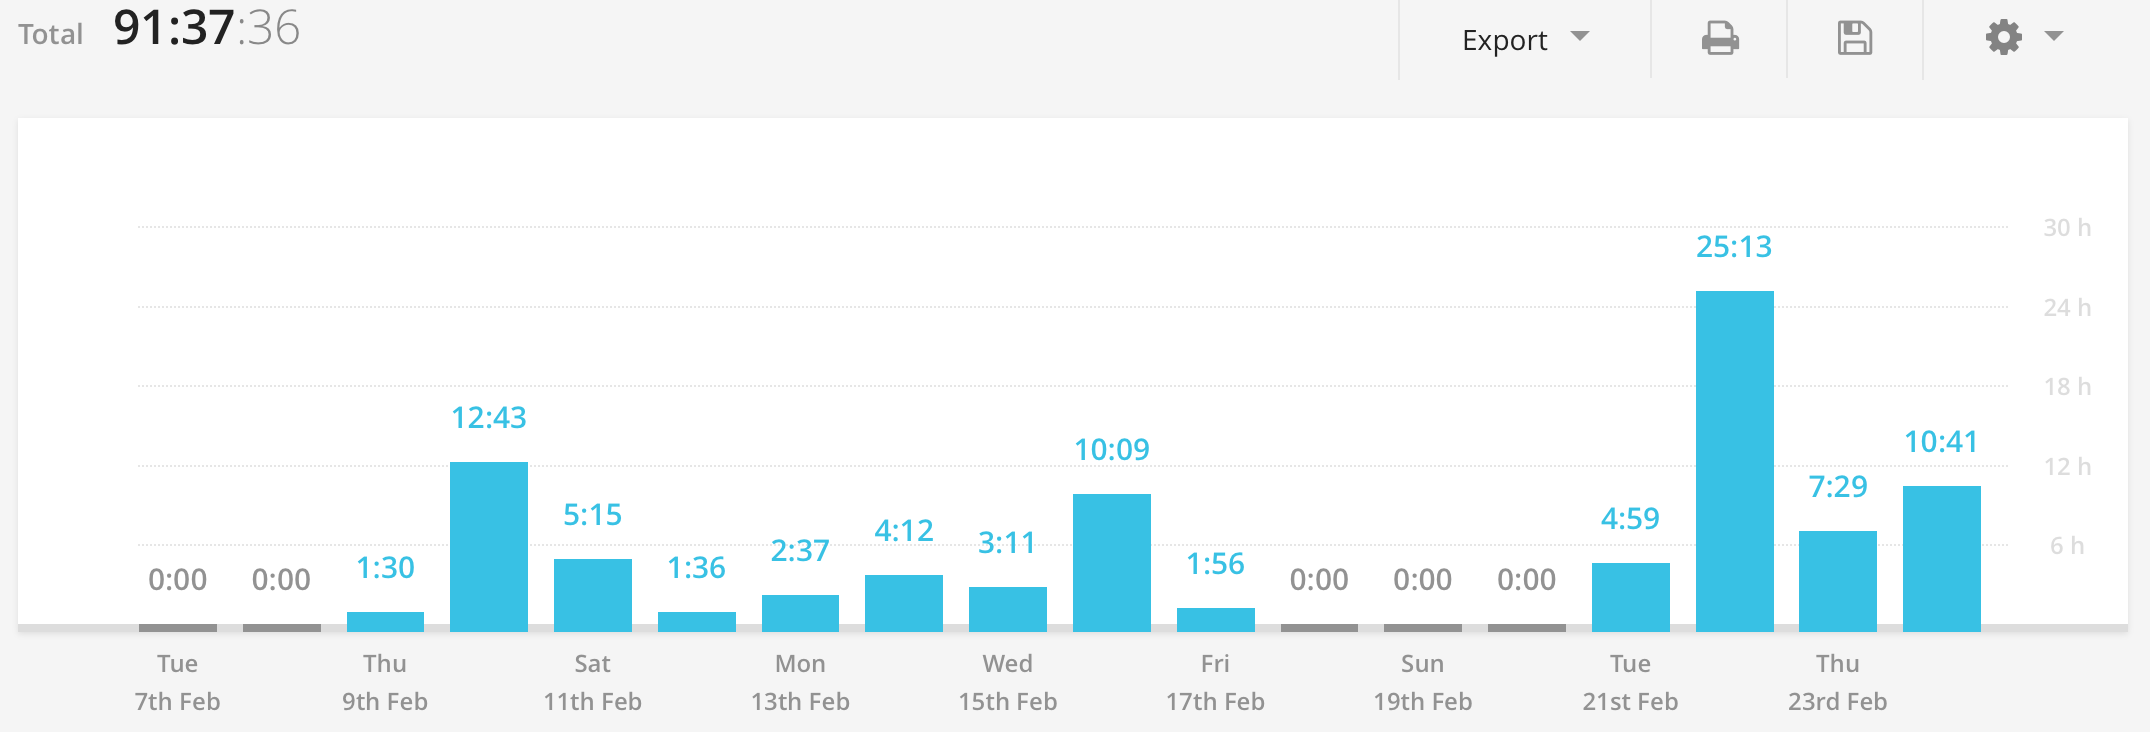
\includegraphics[width=1\textwidth]{./img/horasTotales.png}
\end{center}
\caption{Horas invertidas en total cada día}
\label{tab:horasTotales}
\end{figure}

\begin{figure}[H]
\begin{center}
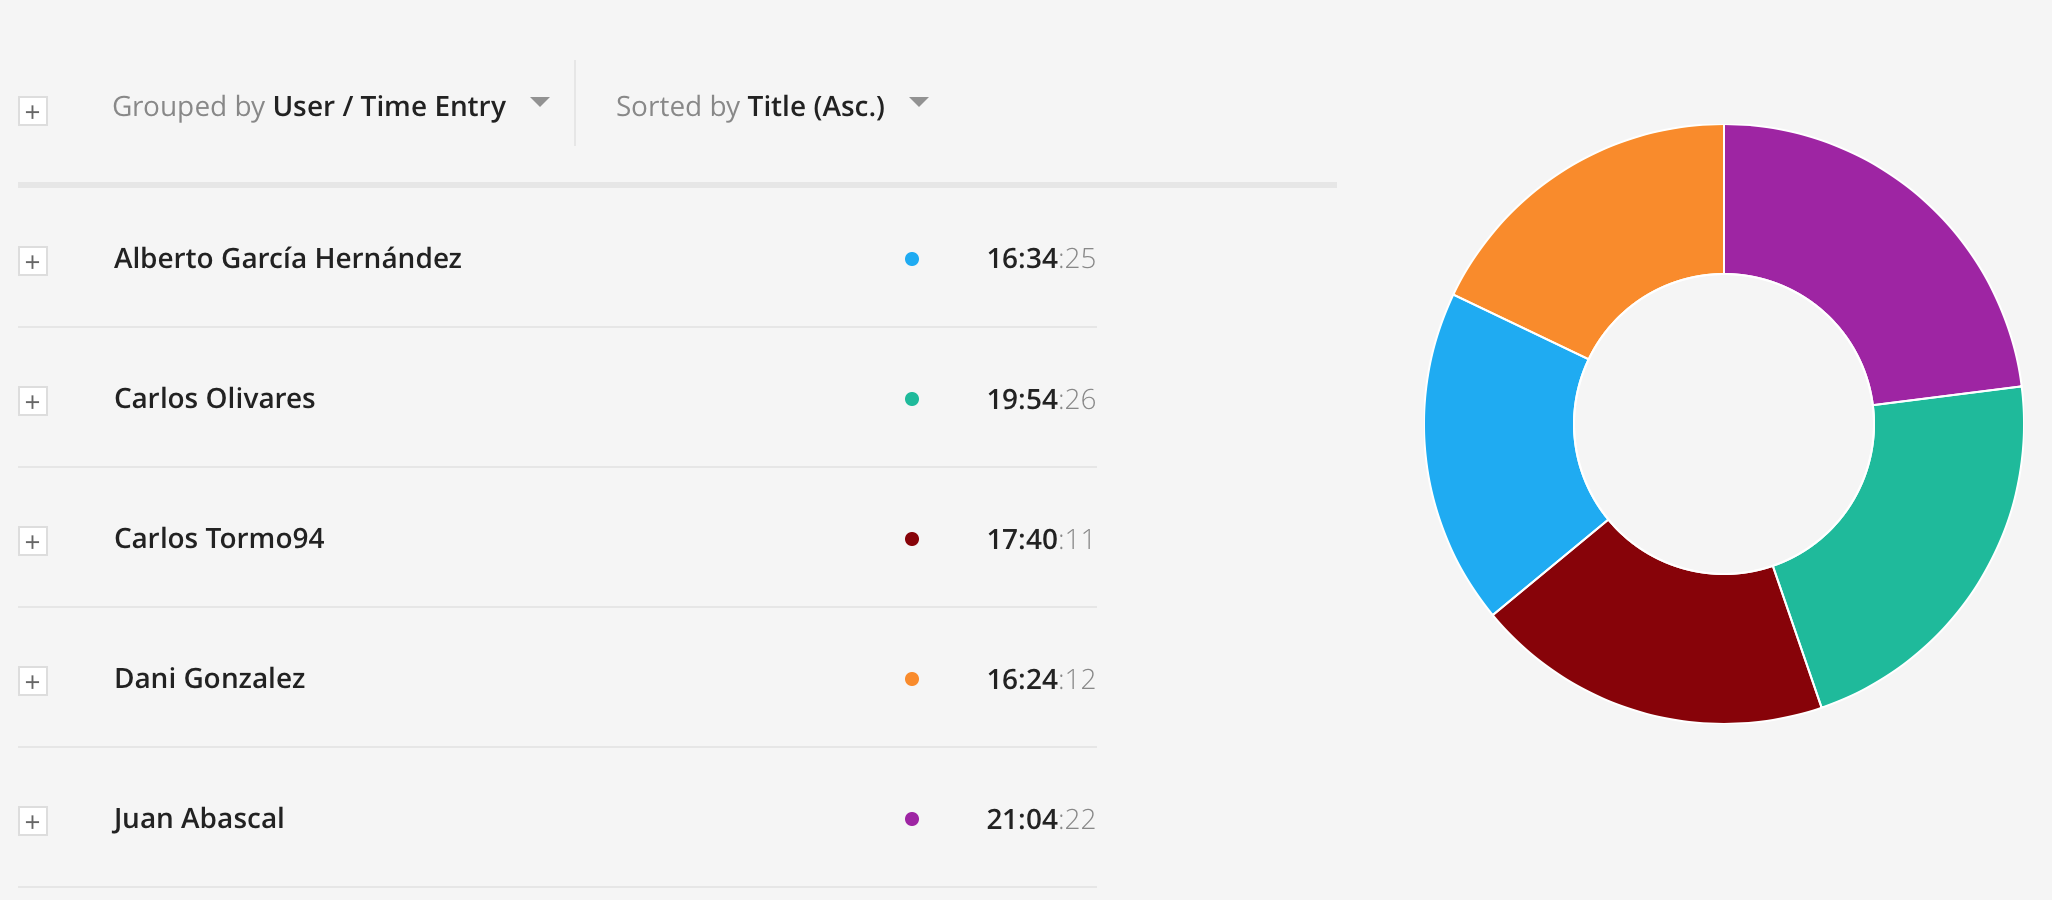
\includegraphics[width=1\textwidth]{./img/horasMiembro.png}
\end{center}
\caption{Horas invertidas por cada miembro del equipo}
\label{tab:horasMiembro}
\end{figure}

\subsection*{Distribución de responsabilidades}
\par Para la gestión de las tareas realizadas y la distribución de las mismas se ha utilizado la herramienta \textit{Trello}. Así, el raparto final de tareas ha sido el mostrado en el cuadro \ref{tabla:respDist}.

\begin{table}[H]
\begin{center}
\begin{tabular}{ l p{9cm} }
\textbf{Nombre}&\textbf{Contribuciones al proyecto}\\
\hline \hline
Alberto García & Secciones 2.1, 2.2, 4.3, 6 \\
\hline
Carlos Olivares & Secciones 4.1, 5.1, 5.2, 6 y revisión de calidad\\
\hline
Carlos Tormo & Secciones 1.1, 1.2, 1.3, 4.3, 6\\
\hline
Daniel González & Secciones 3.1, 3.2, 4.2, 6 \\
\hline
Juan Abascal & Secciones 3.1, 3.2, 4.2 , 6\\
\hline
\end{tabular}
\caption{Distribución de responsabilidades.}
\label{tabla:respDist}
\end{center}
\end{table}
